\documentclass[border=10pt]{standalone}
\usepackage{tikz}\usepackage{amsmath}\usetikzlibrary{arrows.meta,patterns}
\begin{document}
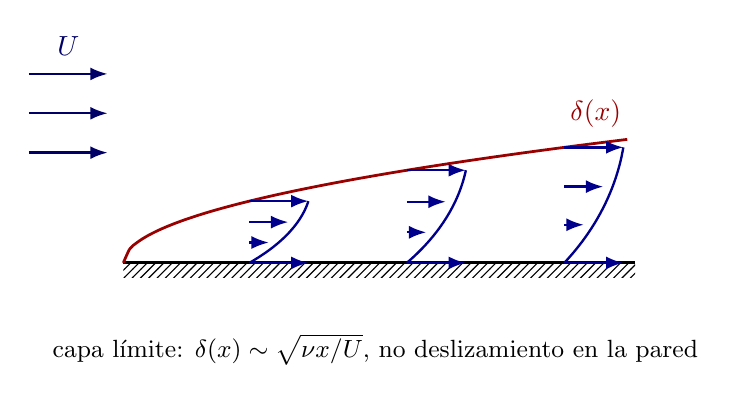
\begin{tikzpicture}[line width=0.85pt,>={Latex[length=2.2mm]}]
  % placa
  \fill[pattern=north east lines] (0,0) rectangle (6.5,-0.18);
  \draw[line width=1.1pt] (0,0)--(6.5,0);
  % flujo libre U
  \foreach \y in {1.4,1.9,2.4} \draw[->,blue!40!black] (-1.2,\y)--(-0.2,\y);
  \node[blue!40!black] at (-0.7,2.75){$U$};
  % borde de la capa limite delta(x) ~ sqrt(x)
  \draw[red!60!black,line width=1pt,domain=0:6.4,samples=80,smooth] plot (\x,{0.62*sqrt(\x)});
  \node[red!60!black] at (6.0,1.9){$\delta(x)$};
  % perfiles de velocidad dentro de la capa
  \foreach \x in {1.6,3.6,5.6}{
    \pgfmathsetmacro{\d}{0.62*sqrt(\x)}
    \draw[blue!55!black] (\x,0) .. controls (\x+0.55,0.4*\d) and (\x+0.7,0.8*\d) .. (\x+0.75,\d);
    \draw[blue!55!black,->] (\x,0.0)--(\x+0.75,0.0);
    \foreach \f in {0.33,0.66,1.0} \draw[blue!55!black,->] (\x,\f*\d)--++({0.75*\f*1.0},0);
  }
  \node at (3.2,-1.1){\small capa límite: $\delta(x)\sim\sqrt{\nu x/U}$, no deslizamiento en la pared};
\end{tikzpicture}
\end{document}
